\documentclass{ltjbook}
\usepackage[ipa]{luatexja-preset}
\usepackage{amssymb,amsfonts}
\usepackage[fleqn]{amsmath}
\usepackage{graphicx}
\usepackage{pifont}
\usepackage{tikz}
\usepackage{bm}
\usetikzlibrary{intersections,calc,arrows.meta,
  decorations.pathreplacing,
  decorations.pathmorphing,
  decorations.text,
  positioning,angles,quotes}
\title{数学図案集}
\author{加藤公一 Kimikazu KATO}
\西暦
\begin{document}
\maketitle
\chapter{ベクトル}
\begin{figure}[ht]\caption{等しいベクトルの例}
\begin{tikzpicture}
  \draw[-Stealth](1,1)--(4,3);
  \draw[-Stealth](3,0)--(6,2);
  \filldraw(1,1)circle(1pt)node[below]{A};
  \filldraw(4,3)circle(1pt)node[right]{B};
  \filldraw(3,0)circle(1pt)node[below]{C};
  \filldraw(6,2)circle(1pt)node[right]{D};
  \draw(2.5,2)node[above left]{$\overrightarrow{\mathrm{AB}}$};
  \draw(4.5,1)node[above left]{$\overrightarrow{\mathrm{CD}}$};
\end{tikzpicture}
\end{figure}
\begin{figure}[ht]\caption{逆ベクトル}
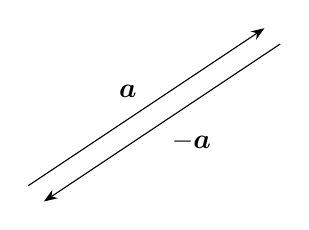
\begin{tikzpicture}
  \draw[-Stealth](1,1)--(4,3)node[midway, above left]{$\bm{a}$};
  \draw[-Stealth](4.2,2.8)--(1.2,0.8)node[midway, below right]{$-\bm{a}$};
\end{tikzpicture}
\end{figure}
\begin{figure}[ht]\caption{ベクトルの実数倍}
\begin{tikzpicture}
  \draw[-Stealth](1,0)--(1+3,2)node[midway, above left]{$\bm{a}$};
  \draw[-Stealth](3,0)--(3+6,4)node[midway, above left]{$2\bm{a}$};
  \draw[-Stealth](6,0)--(6+3/2,1)node[midway, above left]{$\displaystyle\frac{1}{2}\bm{a}$};
  \draw[-Stealth](8,0)--(8-3/2,-1)node[midway, below right]{$\displaystyle-\frac{1}{2}\bm{a}$};
\end{tikzpicture}
\end{figure}
\begin{figure}[ht]\caption{ベクトルの和(その1)}
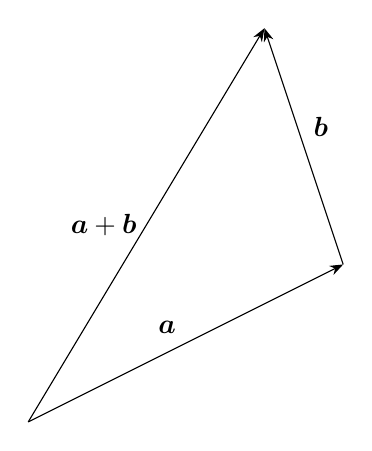
\begin{tikzpicture}
  \draw[-Stealth](0,0)--(4,2)node[midway, above left]{$\bm{a}$};
  \draw[-Stealth](4,2)--(3,5)node[midway, above right]{$\bm{b}$};
  \draw[-Stealth](0,0)--(3,5)node[midway, left]{$\bm{a}+\bm{b}$};
\end{tikzpicture}
\end{figure}
\begin{figure}[ht]\caption{ベクトルの和(その2)}
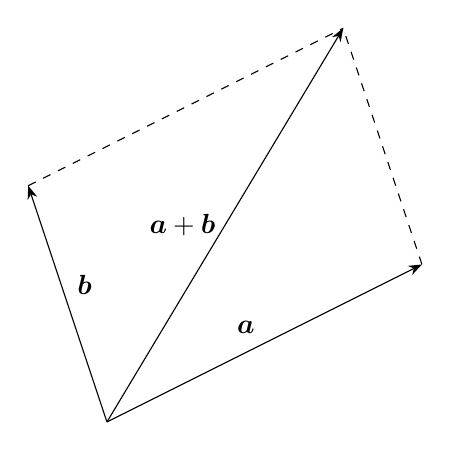
\begin{tikzpicture}
  \draw[-Stealth](0,0)--(4,2)node[midway, above left]{$\bm{a}$};
  \draw[-Stealth](0,0)--(-1,3)node[midway, above right]{$\bm{b}$};
  \draw[-Stealth](0,0)--(3,5)node[midway, left]{$\bm{a}+\bm{b}$};
  \draw[dashed](4,2)--(3,5);
  \draw[dashed](-1,3)--(3,5);
\end{tikzpicture}
\end{figure}
\begin{figure}[ht]\caption{$\bm{a}+\bm{b}=\bm{b}+\bm{a}$}
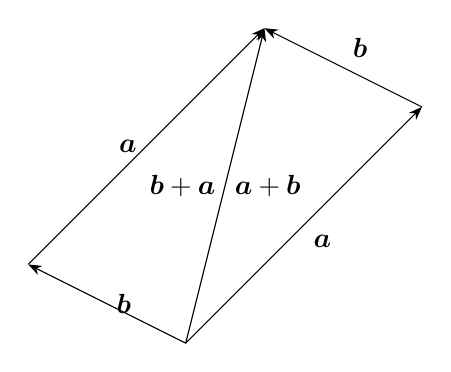
\begin{tikzpicture}
  \draw[-Stealth](1,0)--(4,3)node[midway, below right]{$\bm{a}$};
  \draw[-Stealth](4,3)--(2,4)node[midway, above right]{$\bm{b}$};
  \draw[-Stealth](1,0)--(2,4)node[midway, right]{$\bm{a}+\bm{b}$}node[midway, left]{$\bm{b}+\bm{a}$};
  \draw[-Stealth](1,0)--(-1,1)node[midway, right]{$\bm{b}$};
  \draw[-Stealth](-1,1)--(2,4)node[midway, left]{$\bm{a}$};
\end{tikzpicture}
\end{figure}
\begin{figure}[ht]\caption{$(\bm{a}+\bm{b})+\bm{c}=\bm{a}+(\bm{b}+\bm{c})$}
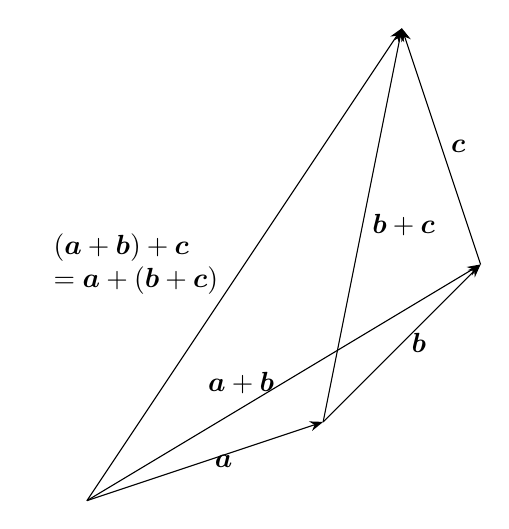
\begin{tikzpicture}
  \draw[-Stealth](0,0)--(3,1)node[midway, right]{$\bm{a}$};
  \draw[-Stealth](3,1)--(5,3)node[midway, right]{$\bm{b}$};
  \draw[-Stealth](5,3)--(4,6)node[midway, right]{$\bm{c}$};  
  \draw[-Stealth](0,0)--(5,3)node[midway, left]{$\bm{a}+\bm{b}$};
  \draw[-Stealth](3,1)--(4,6)node[midway, right]{$\bm{b}+\bm{c}$};
  \draw[-Stealth](0,0)--(4,6)node[midway, left]{
    \begin{tabular}{l}
     $(\bm{a}+\bm{b})+\bm{c}$\\
      $=\bm{a}+(\bm{b}+\bm{c})$
    \end{tabular}};  
\end{tikzpicture}
\end{figure}
\begin{figure}[ht]\caption{ベクトルの大きさ(2次元)}
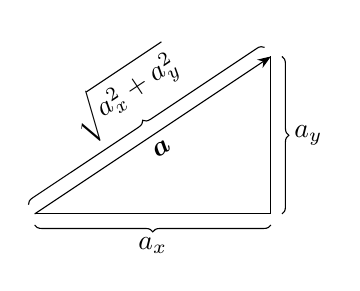
\begin{tikzpicture}
  \draw(3,0)--(0,0)node[midway, below=5pt]{$a_x$};
  \draw[decorate, decoration={brace, raise=4pt}](3,0)--(0,0);
  \draw(3,2)--(3,0)node[midway, right=5pt]{$a_y$};
  \draw[decorate, decoration={brace, raise=4pt}](3,2)--(3,0);
  \draw[decorate, decoration={brace, raise=4pt}](0,0)--(3,2)
  node[midway, sloped, above=5pt]{$\sqrt{a_x^2+a_y^2}$};
  \draw[-Stealth](0,0)--(3,2)node[midway, sloped, below]{$\bm{a}$};
\end{tikzpicture}
\end{figure}
\begin{figure}[ht]\caption{ベクトルの大きさ(3次元)}
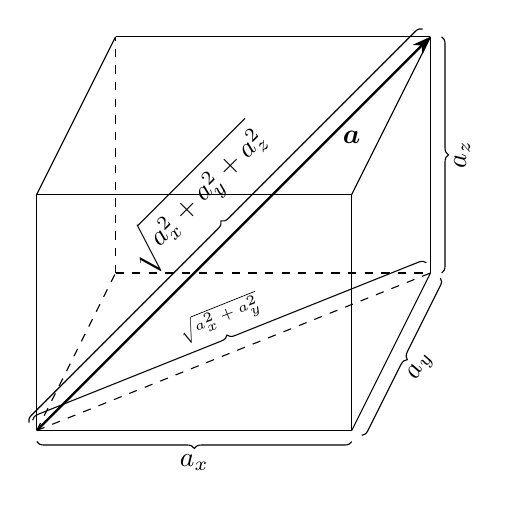
\begin{tikzpicture}
  \draw(0,0)--(4,0)node[midway, below=5pt]{$a_x$};
  \draw[decorate, decoration={brace, raise=4pt}](4,0)--(0,0);
  \draw[dashed](0,0)--(1,2);
  \draw[dashed](1,2)--(1,5);
  \draw(0,0)--(0,3);
  \draw(0,3)--(1,5);
  \draw(0,3)--(4,3);
  \draw(1,5)--(5,5);
  \draw(5,2)--(5,5)node[midway, sloped, below=5pt]{$a_z$};
  \draw[decorate, decoration={brace, raise=4pt}](5,5)--(5,2);
  \draw[dashed](1,2)--(5,2);
  \draw(4,0)--(4,3);
  \draw(4,0)--(5,2)node[midway, sloped, below=5pt]{$a_y$};
  \draw[decorate, decoration={brace, raise=4pt}](5,2)--(4,0);
  \draw(4,3)--(5,5);
  \draw[-Stealth, style=thick](0,0)--(5,5)node[midway, sloped, above=5pt]{$\sqrt{a_x^2+a_y^2+a_z^2}$}node[below=2pt,pos=0.8]{$\bm{a}$};
  \draw[decorate, decoration={brace, raise=4pt}](0,0)--(5,5);
  \draw[dashed](0,0)--(5,2)node[midway, sloped, above=5pt]{\tiny$\sqrt{a_x^2+a_y^2}$};
  \draw[decorate, decoration={brace, raise=4pt}](0,0)--(5,2);
\end{tikzpicture}
\end{figure}


\chapter{三角関数}
\begin{figure}[ht]\caption{$\sin$と$\cos$の定義(その1)}
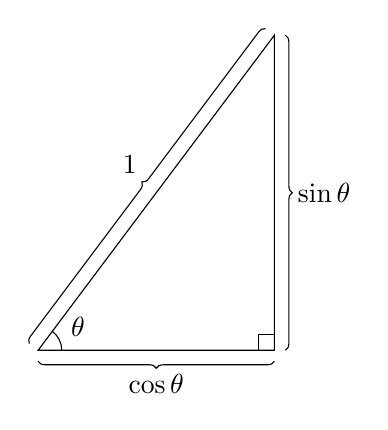
\begin{tikzpicture}
  \coordinate(A) at (0,0);
  \coordinate(B) at (3,0);
  \coordinate(C) at (3,4);
  \coordinate(P) at ($(B)+(-0.2,0.2)$);
  \draw(A)--(B)node[midway,below=5pt]{$\cos\theta$}
  --(C)node[midway,right=5pt]{$\sin\theta$}--cycle node[midway, above left=5pt]{1};
  \draw(P)--($(A)!(P)!(B)$);
  \draw(P)--($(B)!(P)!(C)$);
  \draw(0.3,0)arc(0:{atan(4/3)}:0.3)node[pos=0.2, above right]{$\theta$};
  \draw[decorate, decoration={brace, mirror, raise=4pt}](A)--(B);
  \draw[decorate, decoration={brace, mirror, raise=4pt}](B)--(C);
  \draw[decorate, decoration={brace, mirror, raise=4pt}](C)--(A);
\end{tikzpicture}
\end{figure}
\begin{figure}[ht]\caption{$\sin$と$\cos$の定義(その2)}
\begin{tikzpicture}
  \def\a{55}
  \draw(0,0) circle[radius=2];
  \draw(0,0)-- ++(\a:2)node[right, font=\small]{$(\cos\theta,\sin\theta)$};
  \draw[->](-3,0)--(3,0)node[right]{$x$};
  \draw[-Stealth](0,-3)--(0,3)node[above]{$y$};
  \draw(0,0)node[below left]{0};
  \draw(0.3,0)arc(0:\a:0.3);
  \node[above]at(0.4,0){$\theta$};
  \fill(\a:2)circle[radius=1pt];
  \draw(2,0)node[below right]{$1$};
\end{tikzpicture}
\end{figure}
\begin{figure}[ht]\caption{$-\theta$と$\pi-\theta$についての$\sin$と$\cos$}
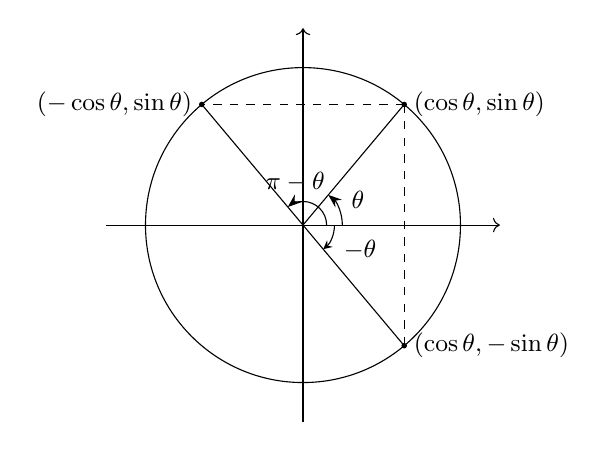
\begin{tikzpicture}
  \def\a{50}
  \draw[->] (-2.5,0)--(2.5,0);
  \draw[->] (0,-2.5)--(0,2.5);
  \draw(0,0)circle[radius=2];
  \draw[-Stealth](0.5,0) arc(0:\a:0.5)
  node[pos=0.2, above right, font=\small]{$\theta$};
  \draw(0,0)--(\a:2);
  \draw[-Stealth](0.3,0) arc(0:180-\a:0.3);
  \node[above, font=\small]at(-0.1,0.3){$\pi-\theta$};
  \draw(0,0)--(180-\a:2);
  \draw[-stealth](0.4,0) arc(0:-\a:0.4)
  node[pos=0.2, below right, font=\small]{$-\theta$};
  \draw(0,0)--(-\a:2);
  \draw[dashed](\a:2)--(-\a:2);
  \draw[dashed](\a:2)--(180-\a:2);
  \fill(\a:2)circle[radius=1pt]node[right,font=\small]{$(\cos\theta,\sin\theta)$};
  \fill(180-\a:2)circle[radius=1pt]node[left,font=\small]{$(-\cos\theta,\sin\theta)$};
  \fill(-\a:2)circle[radius=1pt]node[right,font=\small]{$(\cos\theta,-\sin\theta)$};
\end{tikzpicture}
\end{figure}
\begin{figure}[ht]\caption{$\frac{\pi}{2}-\theta$についての$\sin$と$\cos$}
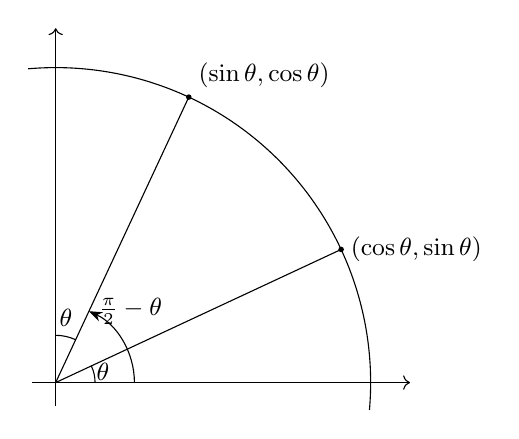
\begin{tikzpicture}
  \def\a{25}
  \draw[->] (-0.3,0)--(4.5,0);
  \draw[->] (0,-0.3)--(0,4.5);
  \draw(-5:4)arc(-5:95:4);
  \draw(0.5,0) arc(0:\a:0.5);
  \node[above, font=\small]at(0.6,-0.1){$\theta$};
  \draw(0,0)--(\a:4);
  \draw[-Stealth](1,0) arc(0:90-\a:1);
  \node[right, font=\small]at(90-\a:1){$\frac{\pi}{2}-\theta$};
  \draw(0,0)--(90-\a:4);
  \draw(90-\a:0.6)arc(90-\a:90:0.6)node[midway,above,font=\small]
  {$\theta$};
  \fill(\a:4)circle[radius=1pt]node[right,font=\small]{$(\cos\theta,\sin\theta)$};
  \fill(90-\a:4)circle[radius=1pt]node[above right,font=\small]{$(\sin\theta,\cos\theta)$};
\end{tikzpicture}
\end{figure}
\begin{figure}[ht]\caption{正弦定理}
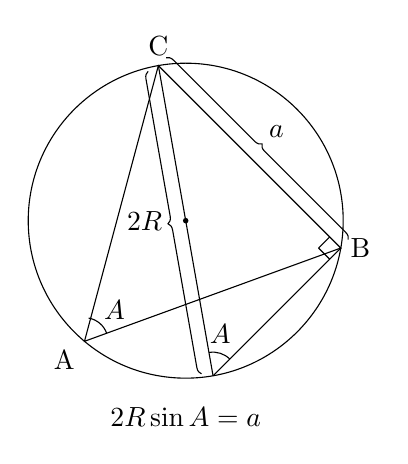
\begin{tikzpicture}
  \def\a{-130}
  \def\b{-10}
  \def\c{100}
  \def\d{\c-180}
  \draw(0,0) circle[radius=2];
  \coordinate(A) at (\a:2);
  \coordinate(B) at (\b:2);
  \coordinate(C) at (\c:2);
  \coordinate(D) at (\d:2);
  \coordinate(P) at ($(B)!0.2cm!(C)!0.2cm!90:(C)$);
  \draw(A)node[below left]{A}--(B)node[right]{B}
  --(C)node[midway, above right=5pt]{$a$}node[above]{C}
  --cycle;
  \draw(C)--(D)node[midway, left=5pt]{$2R$};
  \draw(B)--(D);
  \draw[decorate,
  decoration={brace, mirror, raise=4pt,
    pre=moveto, pre length=0.05cm,
    post=moveto, post length=0.05cm}](C)--(D);
  \draw[decorate, decoration={brace, raise=4pt}](C)--(B);
  \draw(P)--($(C)!(P)!(B)$);
  \draw(P)--($(D)!(P)!(B)$);
  \draw($(D)+({0.3*cos(45)},{0.3*sin(45)})$)arc(45:100:0.3)
  node[midway, above]{$A$};
  \draw($(A)+({0.3*cos(20)},{0.3*sin(20)})$)arc(20:80:0.3);
  \node at ($(A)+({0.3*cos(20)},{0.3*sin(20)})+(0.1,0.3)$) {$A$};
  \fill(0,0)circle[radius=1pt];
  \draw(0,-2.5)node{$2R\sin A=a$};
\end{tikzpicture}
\end{figure}
\begin{figure}[ht]\caption{余弦定理}
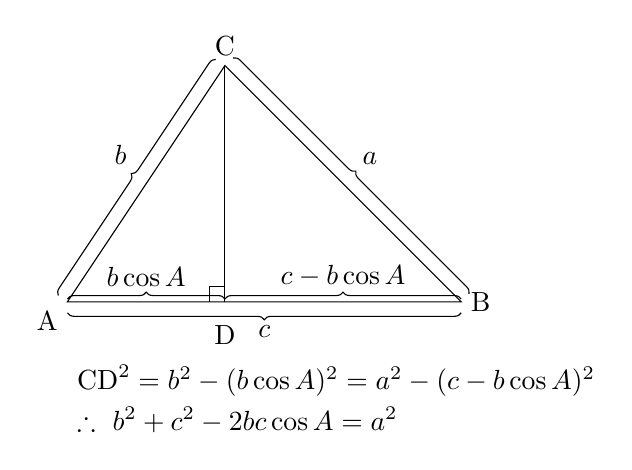
\begin{tikzpicture}
  \coordinate(A) at (0,0);
  \coordinate(B) at (5,0);
  \coordinate(C) at (2,3);
  \coordinate(D) at ($(A)!(C)!(B)$);
  \coordinate(P) at ($(D)+(-0.2,0.2)$);
  \draw(A)node[below left]{A}
  --(B)node[right]{B} node[midway,below=5pt]{$c$}
  --(C)node[above]{C} node[midway,above right=5pt]{$a$}
  --cycle node[midway,above left=5pt]{$b$};
  \draw(C)--(D)node[below=5pt]{D};
  \draw(P)--($(A)!(P)!(D)$);
  \draw(P)--($(C)!(P)!(D)$);
  \draw[decorate, decoration={brace, mirror, raise=4pt}](A)--(B);
  \draw[decorate, decoration={brace, mirror, raise=4pt}](B)--(C);
  \draw[decorate, decoration={brace, mirror, raise=4pt}](C)--(A);
  \draw[decorate, decoration={brace, raise=1pt}](A)--(D);
  \draw[decorate, decoration={brace, raise=1pt}](D)--(B);
  \node at ($(A)!0.5!(D)$) [above=2pt]{$b\cos A$};
  \node at ($(D)!0.5!(B)$) [above=2pt]{$c-b\cos A$};
  \node at (0,-1) [right] {$\mathrm{CD}^2=b^2-(b\cos A)^2=a^2-(c-b\cos A)^2$};
  \node at (0,-1.5) [right] {$\therefore\ b^2+c^2-2bc\cos A=a^2$};
\end{tikzpicture}
\end{figure}
\begin{figure}[ht]\caption{加法定理(その1)}
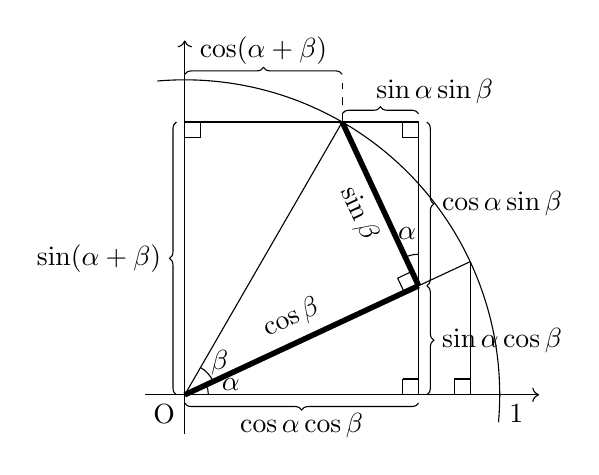
\begin{tikzpicture}
  \def\a{25}
  \def\b{35}
  \draw(-5:4)arc(-5:95:4);
  \draw[->](-0.5,0)--(4.5,0);
  \draw[->](0,-0.5)--(0,4.5);
  \node[below left]at(0,0){O};
  \node[below right]at(4,0){$1$};
  \coordinate(A) at (\a:4);
  \coordinate(B) at ({\a+\b}:4);
  \coordinate(O) at (0,0);
  \coordinate(C) at (A|-O);
  \coordinate(D) at ($(O)!(B)!(A)$);
  \coordinate(E) at (B-|D);
  \coordinate(F) at (E-|O);
  \coordinate(G) at (E|-O);
  \draw[line width=2pt](O)--(D)node[midway, above,sloped]{$\cos\beta$};
  \draw(D)--(A);
  \draw(O)--(B);
  \draw(A)--(C);
  \coordinate(C0) at ($(C)!2mm!(A)!2mm!90:(A)$);
  \draw(C0)--(C0|-C);
  \draw(C0)--(C0-|C);  
  \draw[line width=2pt](B)--(D)node[midway, below,sloped]{$\sin\beta$};
  \coordinate(D0) at ($(D)!2mm!(B)!2mm!90:(B)$);
  \draw(D0)--($(A)!(D0)!(D)$);
  \draw(D0)--($(B)!(D0)!(D)$);
  \coordinate(E0) at ($(E)!2mm!(B)!2mm!90:(B)$);
  \draw(E0)--(E0|-E);
  \draw(E0)--(E0-|E);  
  \draw(E)--(F);
  \draw(E)--(G);
  \coordinate(F0) at ($(F)!2mm!(O)!2mm!90:(O)$);
  \draw(F0)--(F0|-F);
  \draw(F0)--(F0-|F);  
  \coordinate(G0) at ($(G)!2mm!(O)!2mm!-90:(O)$);
  \draw(G0)--(G0|-G);
  \draw(G0)--(G0-|G);
  \pic["$\alpha$", draw, angle eccentricity=2, angle radius=0.3cm]
  {angle=C--O--A};
  \pic["$\beta$", draw, angle eccentricity=1.5, angle radius=0.4cm]
  {angle=A--O--B};
  \pic["$\alpha$", draw, angle eccentricity=1.7, angle radius=0.4cm]
  {angle=E--D--B};
  \draw[decorate, decoration={brace, mirror, raise=3pt}](O)--(G)
  node[midway, below=3pt]{$\cos\alpha\cos\beta$};
  \draw[decorate, decoration={brace, mirror, raise=3pt}](G)--(D)
  node[midway, right=5pt]{$\sin\alpha\cos\beta$};
  \draw[decorate, decoration={brace, mirror, raise=3pt}](D)--(E)
  node[midway, right=5pt]{$\cos\alpha\sin\beta$};
  \draw[decorate, decoration={brace, raise=3pt}](B)--(E)
  node[midway, above right=3pt and -5pt]{$\sin\alpha\sin\beta$};
  \coordinate(B1) at ($(B)+(0,0.5)$);
  \draw[decorate, decoration={brace, raise=3pt}](O|-B1)--(B1)
  node[midway, above=3pt]{$\cos(\alpha+\beta)$};
  \draw[dashed](B)--(B1);
  \draw[decorate, decoration={brace, raise=3pt}](O)--(F)
  node[midway, left=5pt]{$\sin(\alpha+\beta)$};
\end{tikzpicture}
\end{figure}
\begin{figure}[!ht]\caption{加法定理(その2)}
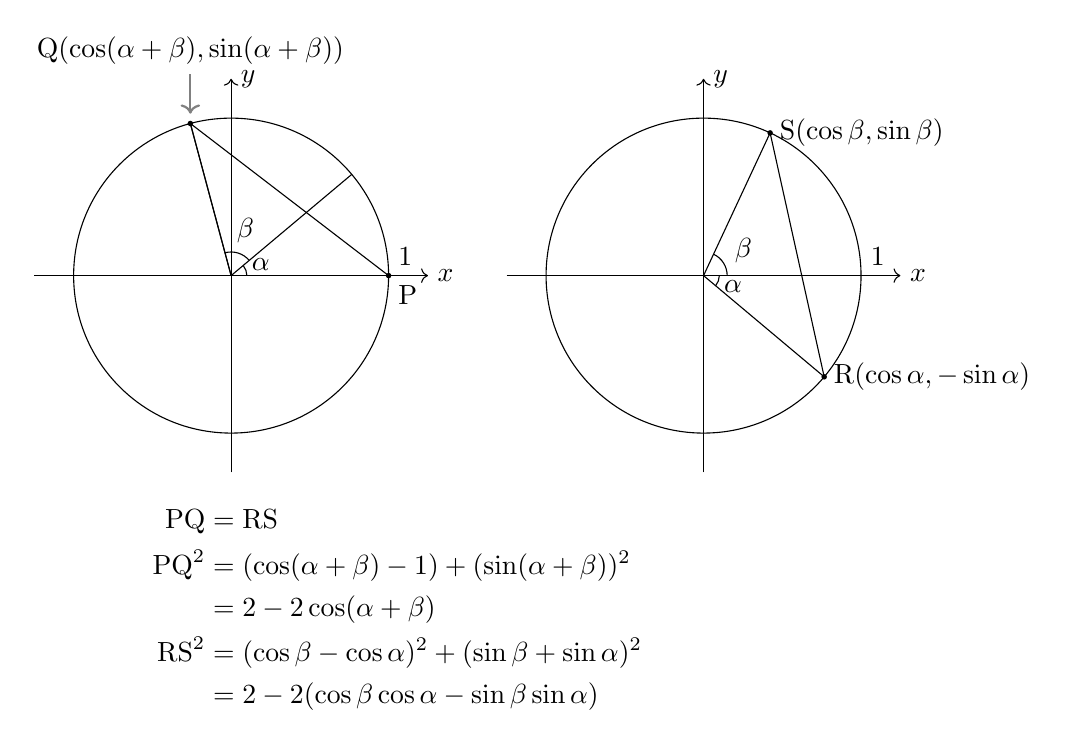
\begin{tikzpicture}
  \def\a{40}
  \def\b{65}
  \def\shift{6}
  \coordinate(O0) at (0,0);
  \coordinate(O1) at (\shift,0);
  \coordinate(A0) at (\a:2);
  \coordinate(P) at (2,0);
  \coordinate(Q) at ({\a+\b}:2);
  \coordinate(R) at ($(-\a:2)+(\shift,0)$);
  \coordinate(S) at ($(\b:2)+(\shift,0)$);
  \coordinate(A1) at ({\shift+2},0);
  \draw(0,0)circle[radius=2];
  \draw[->](-2.5,0)--(2.5,0) node[pos=1, right]{$x$};
  \draw[->](0,-2.5)--(0,2.5) node[pos=1, right]{$y$};
  \draw(\shift,0)circle[radius=2];
  \draw[->]({\shift-2.5},0)--({\shift+2.5},0) node[pos=1, right]{$x$};
  \draw[->](\shift,-2.5)--(\shift,2.5) node[pos=1, right]{$y$};
  \draw(O0)--(A0);
  \draw(O0)--(Q);
  \draw(O0)--(Q);
  \fill(Q)circle[radius=1pt];
  \node[pin={[pin distance=0.5cm, pin edge={<-,thick}]90:
    $\mathrm{Q}(\cos(\alpha+\beta),\sin(\alpha+\beta))$}] at (Q) {};
  \fill(P)circle[radius=1pt]node[below right]{P}node[above right]{$1$};
  \pic["$\alpha$", draw, angle eccentricity=2, angle radius=0.2cm]
  {angle=P--O0--A0};
  \pic["$\beta$", draw, angle eccentricity=2, angle radius=0.3cm]
  {angle=A0--O0--Q};
  \draw(P)--(Q);
  \draw(O1)--(R);
  \draw(O1)--(S);
  \pic["$\alpha$", draw, angle eccentricity=2, angle radius=0.2cm]
  {angle=R--O1--A1};
  \pic["$\beta$", draw, angle eccentricity=2, angle radius=0.3cm]
  {angle=A1--O1--S};
  \fill(R)circle[radius=1pt]node[right]
  {$\mathrm{R}(\cos\alpha,-\sin\alpha)$};
  \fill(S)circle[radius=1pt]node[right]
  {$\mathrm{S}(\cos\beta,\sin\beta)$};
  \node[above right]at(A1){$1$};
  \draw(R)--(S);
  \node[right]at(-2,-4){
    \begin{minipage}[t]{10cm}
    \begin{align*}
      \mathrm{PQ}&=\mathrm{RS}\\
      \mathrm{PQ}^2&=(\cos(\alpha+\beta)-1) + (\sin(\alpha+\beta))^2\\
                 &=2-2\cos(\alpha+\beta)\\
      \mathrm{RS}^2&=(\cos\beta-\cos\alpha)^2+(\sin\beta+\sin\alpha)^2\\
      &=2-2(\cos\beta\cos\alpha-\sin\beta\sin\alpha)
    \end{align*}
    \end{minipage}
  };
\end{tikzpicture}
\end{figure}


\end{document}
